\documentclass[10pt,twocolumn,letterpaper]{article}

\usepackage{cvpr}
\usepackage{times}
\usepackage{epsfig}
\usepackage{graphicx}
\usepackage{amsmath}
\usepackage{amssymb}
\usepackage{mathtools}
\usepackage{alphabeta}
% Include other packages here, before hyperref.

% If you comment hyperref and then uncomment it, you should delete
% egpaper.aux before re-running latex.  (Or just hit 'q' on the first latex
% run, let it finish, and you should be clear).
\usepackage[breaklinks=true,bookmarks=false]{hyperref}

\graphicspath{ {./images/} }

\cvprfinalcopy % *** Uncomment this line for the final submission

\def\cvprPaperID{****} % *** Enter the CVPR Paper ID here
\def\httilde{\mbox{\tt\raisebox{-.5ex}{\symbol{126}}}}

% Pages are numbered in submission mode, and unnumbered in camera-ready
%\ifcvprfinal\pagestyle{empty}\fi
\setcounter{page}{1}
\begin{document}

%%%%%%%%% TITLE
\title{Cycle Generative Adversarial Nets for Style Transfer of Monet Paintings}

\author{Solmaz Mohammadi\\
{\tt\small solmaz.mohammadi@studenti.unipd.it}
% For a paper whose authors are all at the same institution,
% omit the following lines up until the closing ``}''.
% Additional authors and addresses can be added with ``\and'',
% just like the second author.
% To save space, use either the email address or home page, not both
\and
Nicla Faccioli\\
{\tt\small nicla.faccioli@studenti.unipd.it}
}

\maketitle
%\thispagestyle{empty}

%%%%%%%%% ABSTRACT
\begin{abstract}
This article aims at learning the style of the impressionist
painter, Claude Monet. Since the generative adversarial
model has its limitations when it comes to more complex
computer vision problems, we will be using a variation
of generative adversarial models, cycle consistent GAN to capture the
“impression” of an artist from their surroundings. CycleGAN is an unpaired image to image translation using cycle consistent adversarial nets.
\end{abstract}

%%%%%%%%% BODY TEXT
\section{Introduction}
The focus of this paper is to reproduce the style of Claude Monet, the
influential impressionist painter in the nineteenth century. Claude Monet’s style is unique and recognizable by his short and thick strokes that capture the essence of the subject. Monet’s work is particularly interesting because of the strong logarithmic correlations within his paintings that makes it possible to generate new Monet-like images. \cite{monetlog}
This project attempts to transfer the painter's style into existing real-life photos. Style transfer is a computer vision technique that aims to combine two images together. In particular, given a content image (i.e. is interesting for its content) and a style image (i.e. is interesting for its style), the task is to blend them together in order to obtain as output a third image which will represent the content of the first image in the style of the second one. Therefore, we aim to learn a mapping function G: X$\longrightarrow$Y such that the distribution of G(X) is inseparable from the disribution of Y using the adversarial loss (i.e. the discriminator). To further constraint the generator, we pair it with an inverse map F:Y$\longrightarrow$X and use cycle consistency loss to enforce F(G(X))$\sim$X. \cite{cyclegan}
%\\ results

\begin{table*}
	\centering
	\begin{tabular}{c c c c | c c c c}
		\textbf{Real} & 
		\textbf{model1} & 
		\textbf{model2} & 
		\textbf{model3} & 
		\textbf{Real} & 
		\textbf{model1} & 
		\textbf{model2} & 
		\textbf{model3} \\
		&&&&&&&\\
		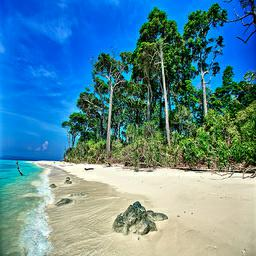
\includegraphics[width=5em]{815_real.jpg}& 
		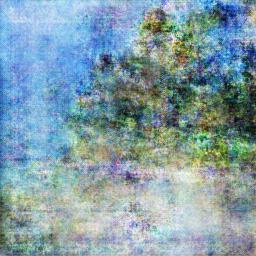
\includegraphics[width=5em]{815_leo.jpg} & 
		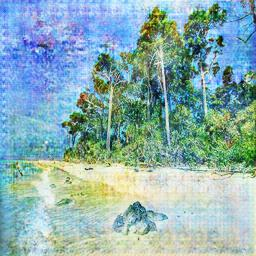
\includegraphics[width=5em]{815_gen.jpg} &
		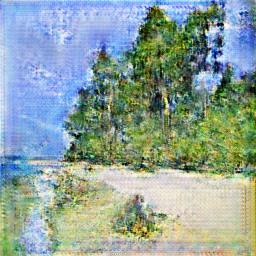
\includegraphics[width=5em]{815_unet.jpg} &
		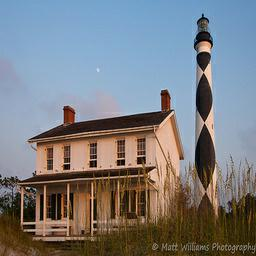
\includegraphics[width=5em]{1326_real.jpg}& 
		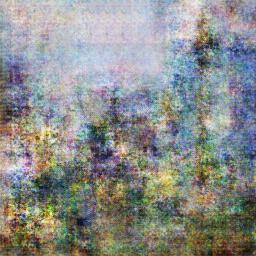
\includegraphics[width=5em]{1326_leo.jpg} & 
		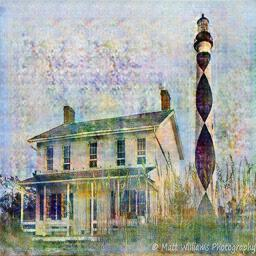
\includegraphics[width=5em]{1326_gen.jpg} &
		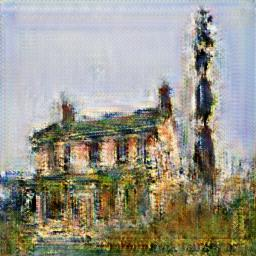
\includegraphics[width=5em]{1326_unet.jpg} \\
		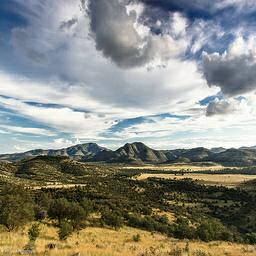
\includegraphics[width=5em]{2378_real.jpg}& 
		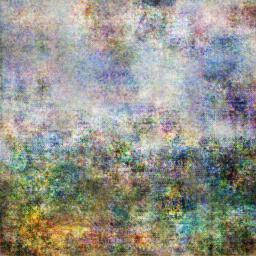
\includegraphics[width=5em]{2378_leo.jpg} & 
		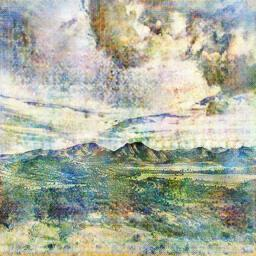
\includegraphics[width=5em]{2378_gen.jpg} &
		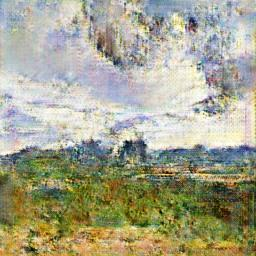
\includegraphics[width=5em]{2378_unet.jpg} &
		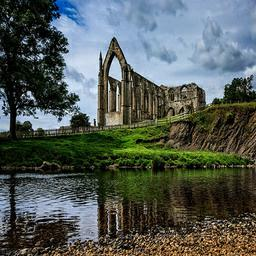
\includegraphics[width=5em]{7033_real.jpg}& 
		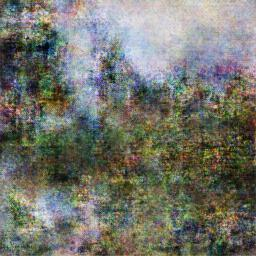
\includegraphics[width=5em]{7033_leo.jpg} & 
		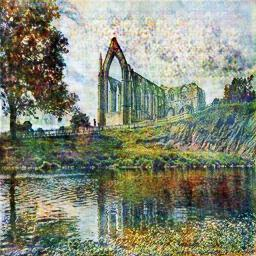
\includegraphics[width=5em]{7033_gen.jpg} &
		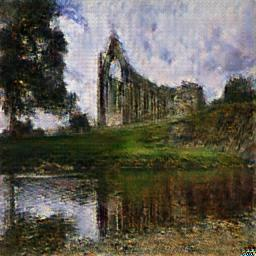
\includegraphics[width=5em]{7033_unet.jpg} \\
		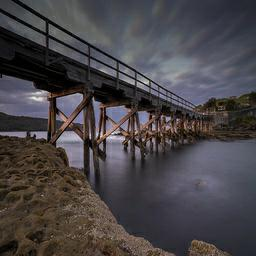
\includegraphics[width=5em]{2605_real.jpg}& 
		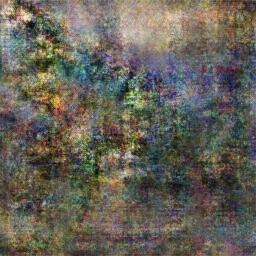
\includegraphics[width=5em]{2605_leo.jpg} & 
		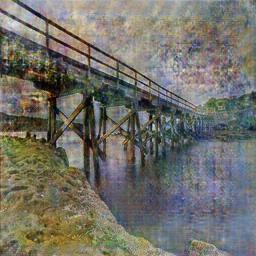
\includegraphics[width=5em]{2605_gen.jpg} &
		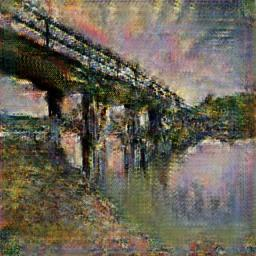
\includegraphics[width=5em]{2605_unet.jpg} &
		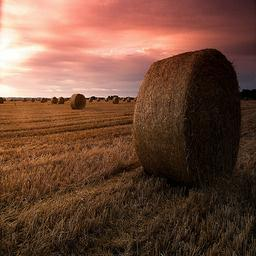
\includegraphics[width=5em]{6476_real.jpg}& 
		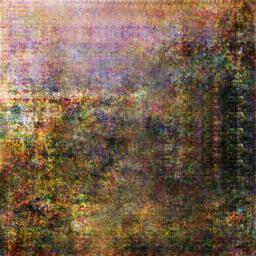
\includegraphics[width=5em]{6476_leo.jpg} & 
		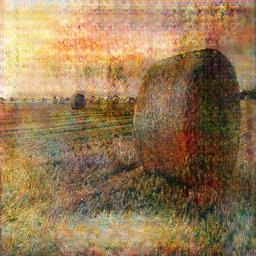
\includegraphics[width=5em]{6476_gen.jpg} &
		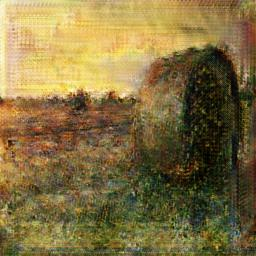
\includegraphics[width=5em]{6476_unet.jpg} \\
	\end{tabular}
	\caption{\textbf{Results}. Comparison between the generated images from different models.}
	\label{table:results}
\end{table*}


\section{Related Work}
In \textbf{Generative Adversarial Nets (GANs)}, two models are trained simultaneously: a generative model G the captures the data distribution, and a discriminative model D that estimates the probability that a sample is from the original data rather than generated by G \cite{simplegan}. The training procedure for G is to maximize the probability of D making a mistake. Therefore, it corresponds to a 2-player minimax problem in which generator tries to “trick” the discriminator. This framework is then the core idea of many generative model applications including cycle consistent GANs. However, the simple GAN is under-constrained for style transfer problem \cite{cyclegan}. We apply a cycle consistency loss objective to further condition GAN.  

\textbf{Paired Image-to-Image Translation}. In some applications the aim is not to generate the image from scratch but rather “translate” an image from a domain X to another domain Y. This can be done by conditioning GAN to learn from a dataset of paired images the function "translating" them. This approach introduces cGAN, where given the input, the output is conditoned by a set of constraints. The conditional GANs learn a mapping from observed data x and random noise vector z, to the output y, G:{x,z}$\rightarrow$y \cite{imgtoimg}.\\
cGANs in the context of image translation can be generalized to cover various problems: image prediction from a map \cite{example1}, future frame prediction \cite{example2}, and image generation from sparse annotations are some examples \cite{example3}. Image-to-Image mappings are also the core idea for style transfer problem but with GAN applied unconditionally \cite{example4}.\\

\textbf{Neural Style Transfer (NST)}. First formulated and demonstrated by \textit{Gatis et al.} \cite{NST}, NST involves the use of a convoutional neural network (e.g., VGG-19) pretrained in object recognition, an image to be transformed (\textit{p}) and an image from which the style has to be copied (\textit{a}). Its goal is to extract the "content representation" of \textit{p} and the  “style representation” of \textit{a} and then to synthetize a new image \textit{x} that will contain both. In a slightly more formal way, it aims to minimize the difference between  \textit{x} and both the content representation of \textit{p} and the style representation of \textit{a}.

\section{Dataset}

The dataset was collected from the competition on Kaggle \cite{kaggle}, a platform in which challenges are proposed and where we got the idea for this project. The dataset is composed by:
\begin{itemize}
\item A set of 300 Monet paintings sized 256x256 in both JPEG and TFRecord format;
\item A set of 7028 photos sized 256x256 in both JPEG and TFRecord format.
\end{itemize}
We used Monet paintings to train our model so that it could learn Monet style and imitate it. Then we applied the learned style over the set of real photos in order to generate new imges that could resemble real paintings. The size of all the images was already the right one for the computation, hence no resizing was needed. 
% data preprocessing

\section{Method}
%discuss your approach for solving the problems that you set up in the introduction. Why is your approach the right thing to do? Did you consider alternative approaches? It may be helpful to include figures, diagrams, or tables to describe your method or compare it with others.
Given the real-life images $\{x_i\}_{i=1}^N$ where $x_{i}\in X$ and monet paintings $\{y_j\}_{j=1}^M$ where $y_{j}\in Y$, donate the data distributions as $x \sim p_{data}(x)$ and $y \sim p_{data}(y)$. We aim to learn the mappings between the two domains $X$ and $Y$ using two generative models $G : X \longrightarrow Y$ and $F : Y \longrightarrow X$. Additionally, we also include two adversarial discriminators $D_{X}$ and $D_{Y}$ where the task of $D_{X}$ is to discriminate between \{x\} and translated images \{F(y)\}. Similarly, $D_{Y}$ aims to distinguish between \{y\} and \{G(x)\} \cite{cyclegan}. The objective of our work is to minimize two losses: \emph{adversarial loss} \cite{simplegan}, which helps to close the gap between the data distribution of target domain and the generated images, and \emph{cycle consistency loss} to keep the results of the two mapping functions consistent.

\subsection{Adversarial Loss}
To learn the distribution of $x \sim p_{data}(x)$, we first define a prior distribution on input noise variables $z \sim p_{z}(z)$ and define a mapping $G(z,\theta)$ where $\theta$ is the set of parameters. The generative model G is often trained using a convolutional neural network \cite{cnn}. We also define a discriminator D (also trained using a CNN) that instead of a single scalar \cite{simplegan}, outputs an image with decreased dimentionality where pixels that are more likely to be in data distribution $p_{data}(x)$ have higher values. We train both models simultaneously in a two-player minimax approach that can be expressed as:
\begin{equation}
	\begin{split}
		\min_G \max_D V(D,G) = &\mathbb{E}_{x \sim p_{data}(x)}[\log{D(x)}]+ \\
		&\mathbb{E}_{z \sim p_{z}(z)}[\log{(1-D(G(z)))}]
	\end{split}
\end{equation}

\subsection{Cycle Consistency Loss}
In theory, adversarial training can fully adapt the target domain distibution and give prominant results. However, real-world datasets can be quite noisy, and in our case the cardinality of the two datasets were considerably uneven. Therefore, the learning process can fail as a network can map the same set of input images to any random permutation of images in the target domain, where any of the learned mappings can induce an output distribution that matches the target distribution \cite{cyclegan}. For this reason, adversarial losses alone cannot guarantee that the desired output is given by the learned function. To further constraint the mapping function, we introduce the \emph{cycle consistency loss}: for each sample $x \in X$, the following cycle $x \rightarrow G(x)\rightarrow F(G(x)) \approx x$ should bring $x$ to the original image. Similarly, for each $y_{i}\in X$, the consistency of $y \rightarrow F(y)\rightarrow G(F(y)) \approx y$ is also satisfied \cite{cyclegan}. The objective is then defined as:
\begin{equation}
	\begin{split}
		\mathcal{L}_{cyc}(G,F) = & \mathbb{E}_{x \sim p_{data}(x)} [\| F(G(x))-x \| _1] + \\
				& \mathbb{E}_{y \sim p_{data}(y)} [\| G(F(y))-y \| _1]
	\end{split}
\end{equation}


\subsection{Implementation}
\textbf{Network Architucture} We used a \textit{U-net CNN} for our generative network. A \textit{U-net} is a fully connected convolutional neural network that was first introduced for biomedical image segmentation \cite{unet}. The standard procedure for our experiments is to first downsample the data (downsampling data is the process of reducing the width and height of the image by strided convolutions), followed by applying several convolutional layers to obtain a deeper image transformation. To generate the final results, we upsample (conversely, increasing the height and width to reach the desired output size) using two convlutional layers with $\frac{1}{2}$ strides. We also applied instance normalization \cite{insnorm} to all layers and established the skip connections in the \textit{Unet}. For the discriminator we used a \text{PatchGAN} model \cite{patchgan}. A \text{PatchGAN} is a type of discriminator for GANs which only penalizes structure at the scale of local image patches. Our PatchGAN discriminator tries to classify if each $30 \times 30$ patch in a given image is real or fake.

\begin{figure}
	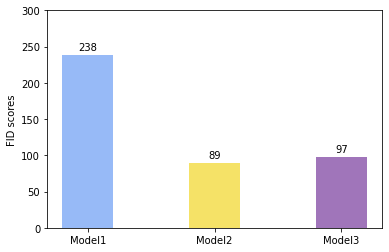
\includegraphics[width=23em]{fid.png}
	\caption{\textbf{FID}. Results of FID evaluated over the different models that we experimented.}
	\label{figure:fid}
\end{figure}

\section{Experiments}
The core of all of our experiments follows the explained objectives and have a fully-connected \textit{U-net} structure. We focused on building different implementations of the \textit{U-net} model and compared the results. Out of all the experiments, we selected three main models: the first model (\texttt{model1}) uses a naive approach in generative models. It has 5 downsampling and 5 upsampling layers with filter size $8 \times 8$ and no intermediate layers. In downsampling, we used \textit{maxpooling} with 2-stride and the activation \textit{leakyReLU}. This model has a high level of noise and the results obtained were not satisfactory. The second model (\texttt{model2}) was inspired by the Kaggle competition suggested framework \cite{kaggle}. It has a smaller filter size ($4 \times 4$) and more layers of both downsampling and upsampling such that it reaches the pixel-sized dimensionality. It uses dropout in three of the upsampling layers and the activation function is \textit{leakyReLU}. This model has the benefit of having more precision as a generator and in some cases generates prominent results. For the third model, (\texttt{model3}) we removed the dropout and instead of reducing the size to 1 pixel in downsampling, we stop at size $64 \times 64$ and added several \textit{transformer} blocks without size alternation. Although this model has a noticeable degree of noise in the generated images, in some examples it is more “monet-esque” to the eyes of the viewers and it contains the brushing style of the painter considerably more than \texttt{model2}. 

\subsection{Evaluation metrics}
In order to evaluate the results of our work we looked for some metrics that could help us in this task \cite{metrics}. To apply them we used already existing code on GitHub \cite{metricsRepo}.

\textbf{Fréchet Inception Distance (FID)}. Introduced by \textit{Heusel et al.} \cite{fid}, FID measures the distance between the feature vector of the generated paintings and the feature vector of the real paintings. Therefore, a lower FID score represents a better performance of the generator since the images it creates are similar to the real ones. The formula to calculate the FID score is the following:
\begin{equation}
	\begin{split}
		\textstyle FID(r, g) = & \| \mu_{r} - \mu_{g} \| _{2}^{2} + \\ 
			& \textstyle Tr(\sum_{r} +  \sum_{g} - 2(\sum_{r}\sum_{g})^\frac{1}{2})
	\end{split}
\end{equation}
 
where $\textstyle (\mu_{r} , \sum_{r})$ is the multivariate normal distribution estimated from a specific layer of Inception Net features for real images and $\textstyle (\mu_{g} , \sum_{g})$ is the multivariate normal distribution estimated from a specific layer of Inception Net features for generated images. 

\textbf{Number of statistically-Different Bins (NDB)}. Introduced by \textit{Richardson and Weiss} \cite{ndb}, this metric is applied to the image pixels and, unlike FID, does not rely on a representation of those images. This evaluation method is based on the observation that given two set of samples originated from the same distribution, the number of samples that falls into a given bin should be the same up to sampling noise. More formally, if $I_{B}(s)$ is an indicator function for bin \textit{B}, i.e. $I_{B}(s)=1$ if the sample \textit{s} falls into bin \text{B} and $I_{B}(s)=0$ otherwise, and given ${s_{i}^{p}}$ and ${s_{j}^{q}}$ respectively ${N_{p}}$ samples from distribution \textit{p} and ${N_{q}}$ samples from distribution q, then if $p=q$ then we expect to be $\textstyle \frac{1}{N_p}\sum_{i}{I_B(s_{i}^{p})} \approx \frac{1}{N_q}\sum_{j}{I_B(s_{j}^{q})} $. When this is not true for a given bin, they are said to be \textit{statistically different}. The test is performed on all bins and then the number of statistically-different bins divided by the number of bins is the final result. We used this metric in order to measure the diversity of the generated images and to understand if the model was encountering mode collapse by generating similar images. 

\textbf{Jensen-Shannon Divergence (JSD)} As reported in \cite{jsd}, JSD is a smoothed and simmetrized version of the Kullback divergence amd measures the divergence between two probability distributions $p$ and $q$. It is defined as: 
\begin{equation}
	\begin{split}
		D_{JS}(p\|q) = \frac{1}{2}D_{KL}(p\|\frac{p+q}{2})+  \frac{1}{2}D_{KL}(q\|\frac{p+q}{2}))
	\end{split}
\end{equation}
This can be used in order to understand the diversity of the generated in a slightly different way with respect to NDB.


\begin{figure}
	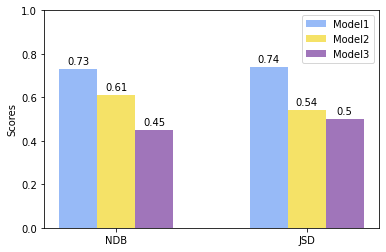
\includegraphics[width=23em]{index.png}
	\caption{\textbf{NDB and JSD}. Results of NDB and JSD evaluated over the different models that we experimented.}
	\label{figure:ndb-jsd}
\end{figure}

\section{Conclusions}
We applied the three models we implemented to the original photos and, as it's possible to see in Table [\ref{table:results}], the results differ a lot from one model to the other. From a visual point of view, the first model we proposed generates output with a huge degree of noise. Hence the result is a set of images in which is impossible to distinguish any element of the original photos. \texttt{Model2} on the other hand is able to generate images that better represent the content of the original photos and also applies some of Monet style. With respect to \texttt{model1}, with \texttt{model2} it is possible to appreciate a relevant improvement. Finally, the third model enhance a bit more the painter style since it's possible to appreciate some hint of strokes and brushing. The issue with \texttt{model3} is that a certain degree of noise is introduced but overall seems to create images that better imitate the orginal paintings. Also the measurment performed by the metrics we applied seems to confirm what we were able to visually appreciate: the quality of the image results are better for \texttt{model2} since it presents a lower level of noise, but from a diversity point of view, \texttt{model3} performed the best. 

{\small
\bibliographystyle{ieee_fullname}
\bibliography{egbib}
}

\end{document}
